%!TEX root = main.tex

\section{Streaming protocol}
\label{sec:control}


Finally, we describe \name's streaming protocol. %, including its real-time quality adaptation algorithm that optimizes the user-perceived quality and how to implement it over existing DASH protocols. 
We focus on two questions: 
(1) how to adapt quality levels, spatially and temporally, to optimize the user-perceived quality in the presence of noises in user actions (\S\ref{subsec:adaptation}); and
(2) how to implement the \name adaptation logic over existing DASH protocols (\S\ref{subsec:compatible}).

\subsection{Robust quality adaptation}
\label{subsec:adaptation}
The \name adapts quality in two levels: {\em chunk-level} quality adaptation and {\em tile-level} quality adaptation. 
The chunk-level adaptation determines the total bitrate of the next chunk to meet buffer length target under the predicted bandwidth.
\name uses BOLA~\cite{bola}, one of the most popular bitrate adaptation algorithms, as the chunk-level adaptation. 

Within each chunk, the tile-level adaptation determines the quality level of each tile to maximize the perceived quality while ensuring the total size of the tiles does not exceed the bitrate of the chunk. 
Suppose the bitrate of a chunk $\Chunk$ is $\Bitrate_\Chunk$. The goal of the tile-level adaptation is to determine for each tile $\Tile\in\Chunk$ the quality level $\Quality_\Tile$, such that the total tile size of these tiles $\sum_{\Tile\in\Chunk}\Quality\leq \Bitrate_\Chunk$, and the total PSPNR $\sum_{\Tile\in\Chunk}\Area_\Tile\PSPNR_\Tile(\Quality_\Tile)$ is maximized. 
Here, the PSPNR of a tile $\Tile$ is weighted by its area $\Area_\Tile$.
Following the assumption that PSPNR is a linear function of quality level (\S\ref{sec:tiling}), we can rewrite the objective as max $\sum_{\Tile\in\Chunk}\Area_\Tile\Efficiency_\Tile\Quality_\Tile$, where $\Efficiency_\Tile$ is the efficiency score of tile $\Tile$. 
Although this is a linear optimization problem, its variable a discrete (quality level), which makes it a mix-integer programing problem. 
\name solves above problem with \fillme, an efficient approximation algorithm. \jc{Guan Yu: please briefly describe the solution}

It is important to notice that that formulation is sensitive to the accuracy of PSPNR, which depends heavily on the knowledge of user action, especially the three new quality-determining factors (\S\ref{sec:opportunities}).
Therefore, the tile-level adaptation seem very susciptible to the prediction errors of user actions, which are fundamentally difficult to predict accurately.

Suprisingly, however, one can achieve a reasonable robustness to the prediction errors of user actions with a simple prediction heuristics. 
The key insight is that although it is indeed hard to predict user actions accurately, it is possible to predict the {\em range} of user actions (\eg at least how fast the viewpoint will be in the next second). 
Figure~\ref{speed_analysis} shows an example of predicting the viewoint moving speed by \fillme. \jc{Guan Yu, what's the heuristics to predict the ``lower bound''?} 
Now, a reliable prediction on the lower bound of PSPNR of a tile is actually sufficient to determine the quality level of a tile because of the ``threshold'' effect of JND on PSPNR; \eg as long as the viewpoint moving speed is above some threshold, the difference between two quality levels would drop dramatically.

\begin{figure}
  \centering
  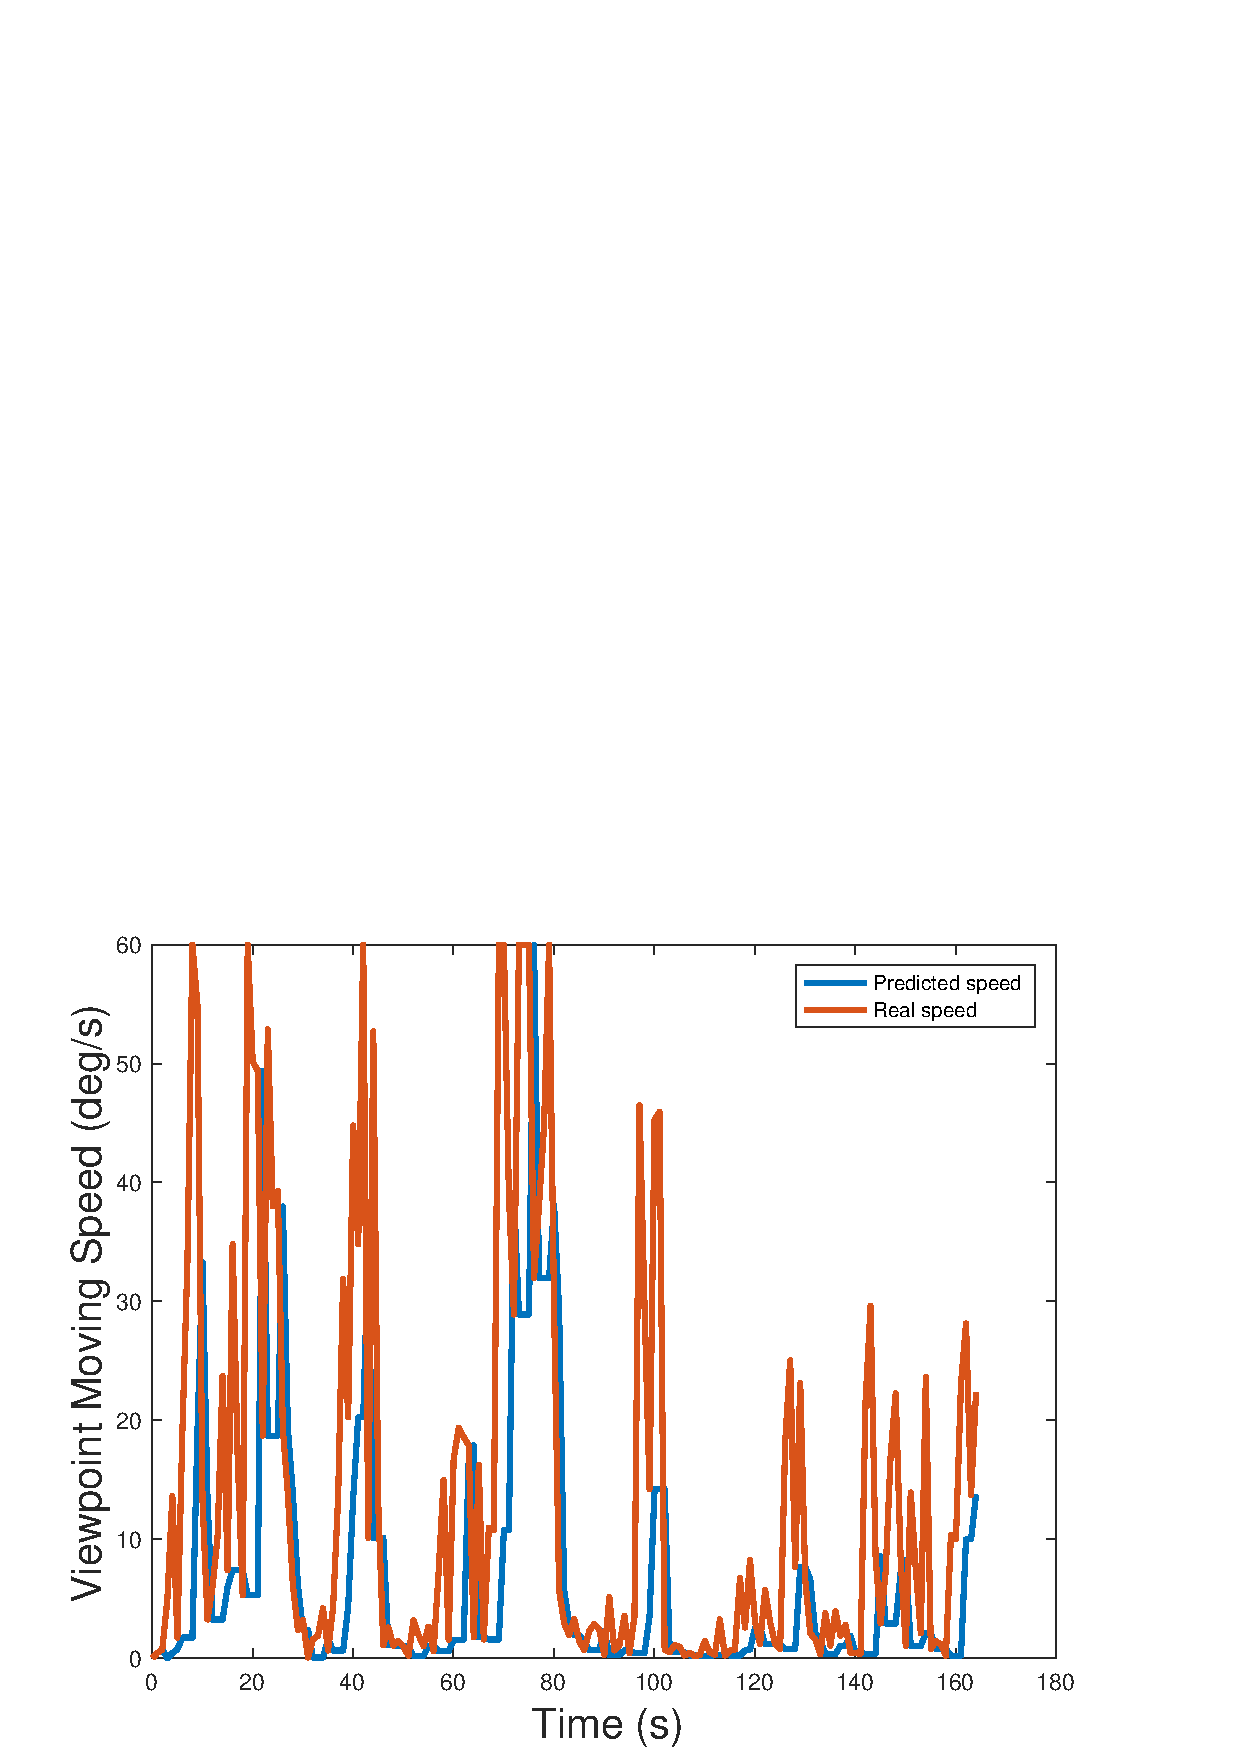
\includegraphics[width=2.5in, height=1in]{images/speed_analysis.pdf}
  \caption{An example of real viewpoint moving pattern and predicted viewpoint moving pattern.}
  \label{speed_analysis}
  \end{figure}


\subsection{DASH-compatible design}
\label{subsec:compatible}